% Packages %%%%%%%%%%%%%%%%%%%%%%%%%%%%%%%%%%%%%%%%%%%%%%%%%%%
\documentclass[conference]{IEEEtran}
\IEEEoverridecommandlockouts 
\usepackage{cite}
\usepackage[cmex10]{amsmath}
\usepackage{amssymb}
%\usepackage{algorithmic}
\usepackage{array}
\usepackage{mdwmath}
\usepackage{mdwtab}
\usepackage{eqparbox}
\usepackage{graphicx}
\usepackage[]{subfigure}
\usepackage{url}
\usepackage[algoruled,vlined,linesnumbered]{algorithm2e}
\usepackage{verbatim}

\makeindex 
\makeatletter

%%%%%%%%%%%%%%%%%%%%%%%%%%%%%%%%%%%%%%%%%%%%%%%%%%%%%%%%%%%%%%%%
% Magic stuff to shrink stuff
\makeatletter
\renewcommand\section{\@startsection{section}{1}{\z@}
                                  {-3.0ex plus -1.5ex minus -0.5ex}
                                  {0.7ex plus 1ex minus 0ex}
                                  {\bfseries}}
\renewcommand\subsection{\@startsection{subsection}{1}{\z@}
                                  {-2.0ex plus -1.5ex minus -0.5ex}
                                  {0.7ex plus 1ex minus 0ex}
                                  {\itshape\bfseries}}
\makeatother


%\newcommand{\shrinka}{\def\baselinestretch{0.99}\large\normalsize}

\long\def\IGNORE#1{}

%%%%%%%%%%%%%%%%%%%%%%%%%%%%%%%%%%%%%%%%%%%%%%%%%%%%%%%%%%%%%%%%%%%
% New commands
\newcommand{\Disks}{\ensuremath{\mathcal{D}}}
\newcommand{\Container}{\ensuremath{\mathit{C}}}
\newcommand{\initMax}{r_{0}\_\text{\textit{Max}}}
\newcommand{\initMin}{r_{0}\_\text{\textit{Min}}}

%%%%%%%%%%%%%%%%%%%%%%%%%%%%%%%%%%%%%%%%%%%%%%%%%%%%%%%%%%%%
% Paper Info
\author{Ana Huam\'{a}n Quispe}
\title{ {CS 6491} {P}roject 4 - Hamiltonian Path Animation}
  
%%%%%%%%%%%%%%%%%%%%%%%%%%%%%%%%%%%%%%%%%%%%%%%%%%%%%%%%%%%%
% Document
\begin{document}
\maketitle

%%%%%%%%%%%%%%%%%%%%%%%%%%%%%%%%%%%%%%%%%%%%%%%%%%%%%%%%
% Abstract
%\abstract{}

%%%%%%%%%%%%%%%%%%%%%%%%%%%%%%%%%%%%%%%%%%%%%%%%%%%%%%%%%%%%%%%%%
% ProblemStatement
\section{Problem Statement}
\label{sec:Problem}
\begin{itemize}
\item{Given a manifold mesh, perform a Hamiltonian traversal by using the Laced Ring algorithm \cite{gurung2011lr} discussed in class.} 
\item{Animate the path creation procedure.}
\end{itemize}

%%%%%%%%%%%%%%%%%%%%%%%%%%%%%%%%%%%%%%%%%%%%%%%%%%%%%%%%%%%%%%%%
\section{Hamiltonian Path}
\label{sec:Approach}

% *****************************
\subsection{Laced Ring Algorithm}
In order to create a path that passed through all the vertices of a given manifold mesh, we implemented a Hamiltonian path using the Laced Ring algorithm. The basic algorithm is shown in Procedure \ref{proc:ringExpander}. As it can be seen, it consists of a greedy invasion of the mesh triangles starting from a random seed corner $s$. The path generated is edge-connected.
% -----------------------------------------
\begin{procedure}[h]

$c = s$ \;
$c.n.v.m = c.p.v.m =$ \ArgSty{true} \;
\Repeat{ $c!= s.o$ }{
\If{ $!c.v.m$ }{
$c.v.m = c.t.m =$ \ArgSty{true} \;
}
\ElseIf{$!c.t.m$}{
$c = c.o$ \;
}
$c = c.r$ \; 
}
\caption{ \FuncSty{ringExpander}($s$) }
\label{proc:ringExpander}
\end{procedure}

% *****************************
\subsection{Implementation Details}
\begin{itemize}
\item{We used the standard Corner Table data structure to save the mesh information. However, we added extra vectors to save new data available:
\begin{itemize}
\item{Marked triangles: Triangles that belonged to the Hamiltonian path}
\item{Triangle type: A vector that stored the type of each Marked Triangle ($T_{0}$, $T_{1}$ or $T_{2}$)}
\end{itemize}
}
\end{itemize}

%%%%%%%%%%%%%%%%%%%%%%%%%%%%%%%%%%%%%%%%%%%%%%%%%%%%%%%%%%%%%%%%
\section{Animation}
\label{sec:Approach}

% *****************************
\subsection{Branch-based path representation}
The Hamiltonian path obtained in the previous section is a tree of triangles with multiple branches.
In order to animate this path as a volumetric curve, we calculated and stored the baricenter of each Marked triangle (triangles on the path). Our base approach consists on simply forming a curve that passes
through these points.

The first problem, of course, comes with the fact that the path branchs off at some triangles, hence the curve cannot be obtained by simply concatenating all the baricenters. To overcome this, we noticed 2 important things:

\begin{itemize}
\item{The Hamiltonian path, obtained with the LR algorithm, grows branches on the points corresponding to triangles of the type $T_{0}$, that is, triangles whose edges are shared with other path triangles}
\item{Starting at a triangle $T_{0}$ on the Hamiltonian path obtained with LR, we reach the end triangle of a branch if and only if this end triangle is of type $T_{2}$ (has 2 shared edges with no-path triangles) }
\end{itemize}

With these observations in mind, our approach for animating will express the Hamiltonian path as a set of branches which start at baricenters of triangles of type $T_{0}$ and end in corresponding baricenters of triangles $T_{2}$:

\begin{itemize}
\item{For all baricenters of the Marked triangles
\begin{itemize}
\item{If the corresponding triangle is of type $T_{0}$, follow the Hamiltonian path (stored in Marked Triangles); adding the traversed baricenter points in a vector $p$. This will represent a new branch of our path. }
\item{End the traverse, once the corresponding triangle is of type $T_{2}$}
\item{Store $p$ as a branch}
\end{itemize}
}
\end{itemize} 

% -------------------------------
% Sphere
\begin{figure}[h]
\centering
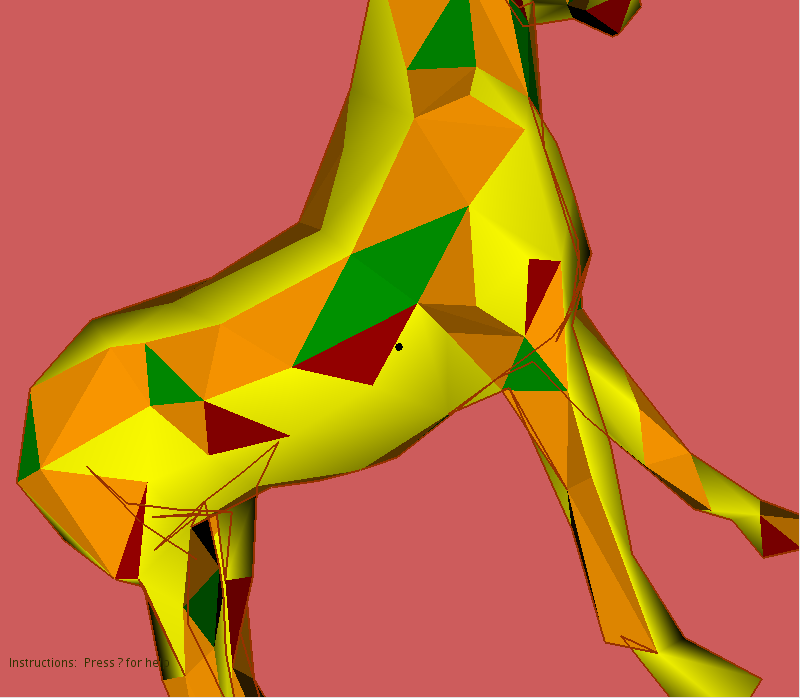
\includegraphics[height=100pt]{images/trianglesT02.png} 
\label{fig:trianglesT02}		
\caption{Example of triangles $T_{0}$ and $T_{2}$ (depicted in green and red respectively)}
\end{figure}

% *****************************
\subsection{Visualization}
The visualization of our Hamiltonian path consists on showing all the branches found in the previous step. For this purpose, we use the Frenet-Serret formulas for each branch (which is after all a curve). We depict the branches as curves that have a circular section at each baricenter point. These sections are located in the plane formed by the Normal and Binormal vector of each corresponding point. Then, we only join these sections and a volume is formed.

For this section we reused part of the base code given in class, which was modified to include visualizing the different branches and the animation procedure.

%%%%%%%%%%%%%%%%%%%%%%%%%%%%%%%%%%%%%%%%%%%%%%%%%%%%%%%%%%%%%%%%
\section{Results}
\label{sec:Results}
Results of our approach using 3 different kind of meshes are shown in the following figures:

% -------------------------------
% Sphere
\begin{figure}[h]
		\centering
		  \subfigure[Hamiltonian path]{
		   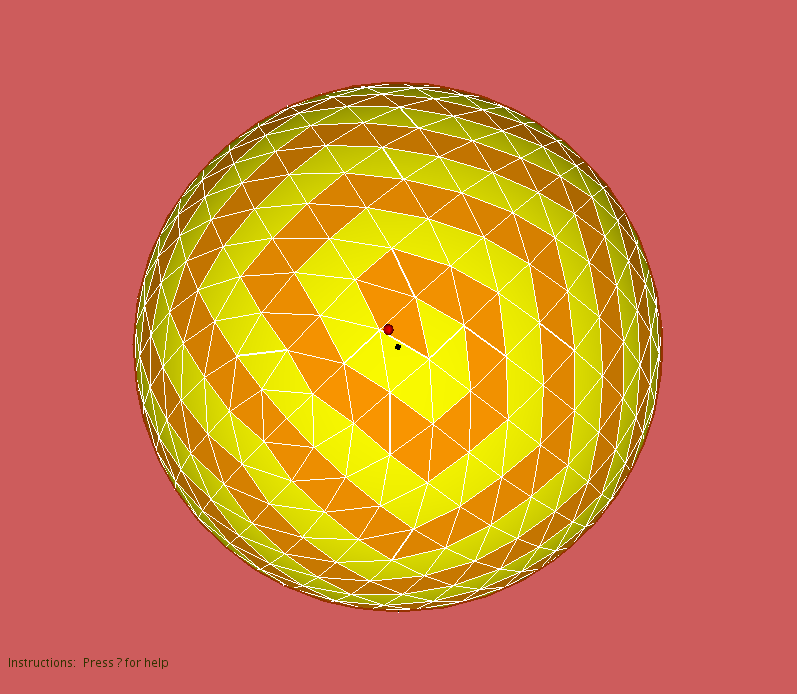
\includegraphics[height=80pt]{images/sphere_path.png} 
		   \label{fig:spherePath}
          }		
		  \subfigure[Animation]{
		   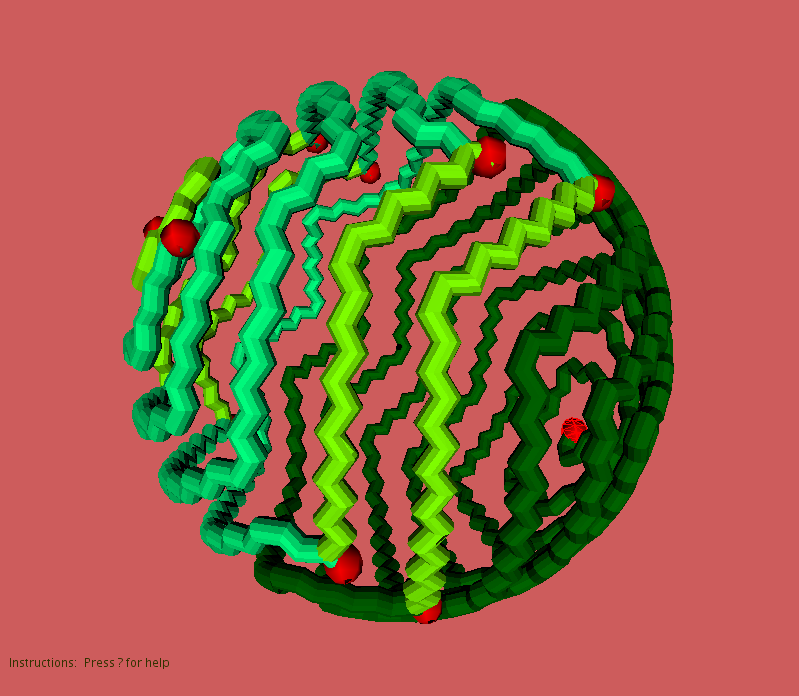
\includegraphics[height=80pt]{images/sphere_pathAnimated.png} 
		   \label{fig:spherePathAnimated}
          }
          \caption{Results with sphereSmooth.vts}
          \label{fig:sphereResult}
\end{figure}


% -------------------------------
% Horse
\begin{figure}[h]
		\centering
		  \subfigure[Hamiltonian path]{
		   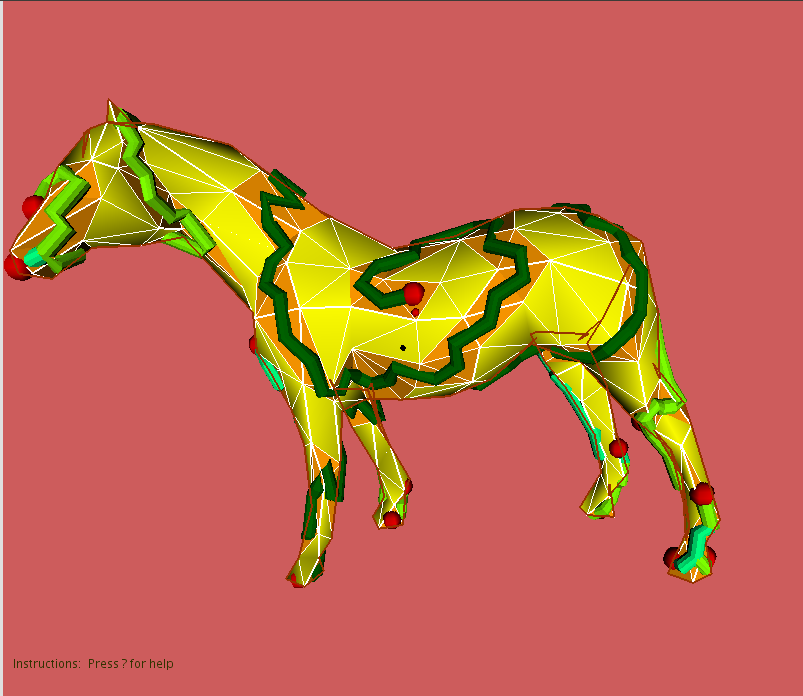
\includegraphics[height=80pt]{images/horse_path.png} 
		   \label{fig:horsePath}
          }		
		  \subfigure[Animation]{
		   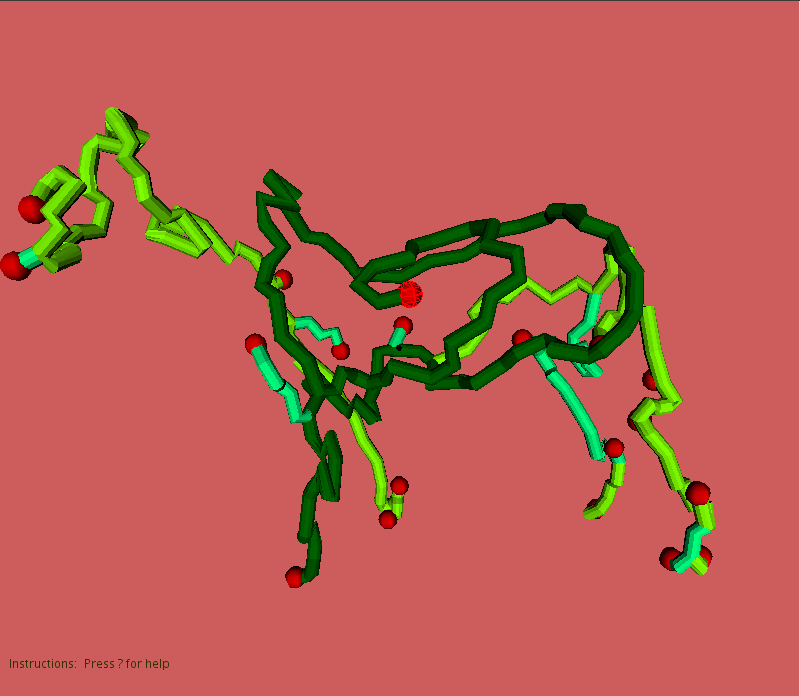
\includegraphics[height=80pt]{images/horse_pathAnimated.png} 
		   \label{fig:horsePathAnimated}
          }
          \caption{Results with horse.vts}
          \label{fig:horseResult}
\end{figure}

% -------------------------------
% Bunny Front
\begin{figure}[h]
		\centering
		  \subfigure[Hamiltonian path (bunny front view)]{
		   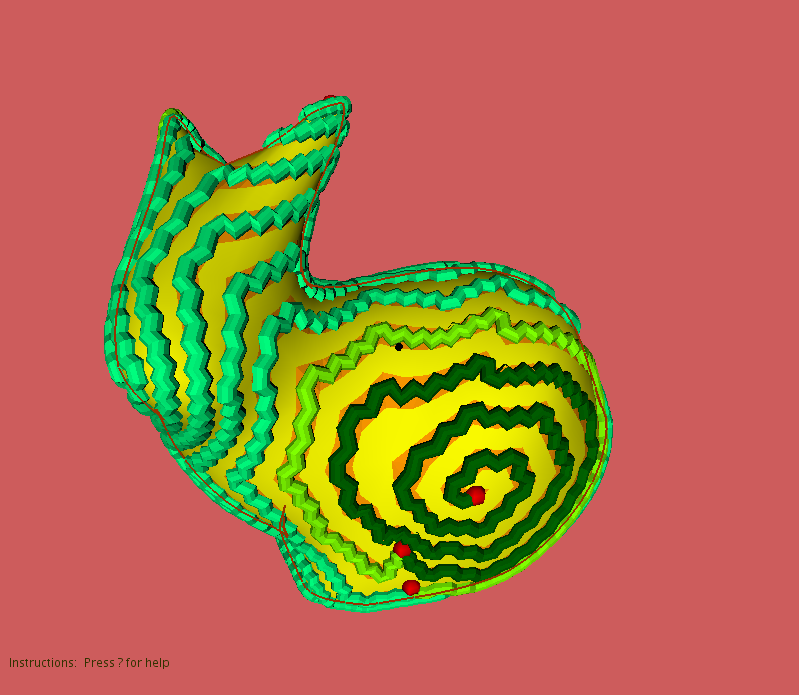
\includegraphics[height=80pt]{images/bunnyFront_path.png} 
		   \label{fig:bunnyFrontPath}
          }		
		  \subfigure[Animation]{
		   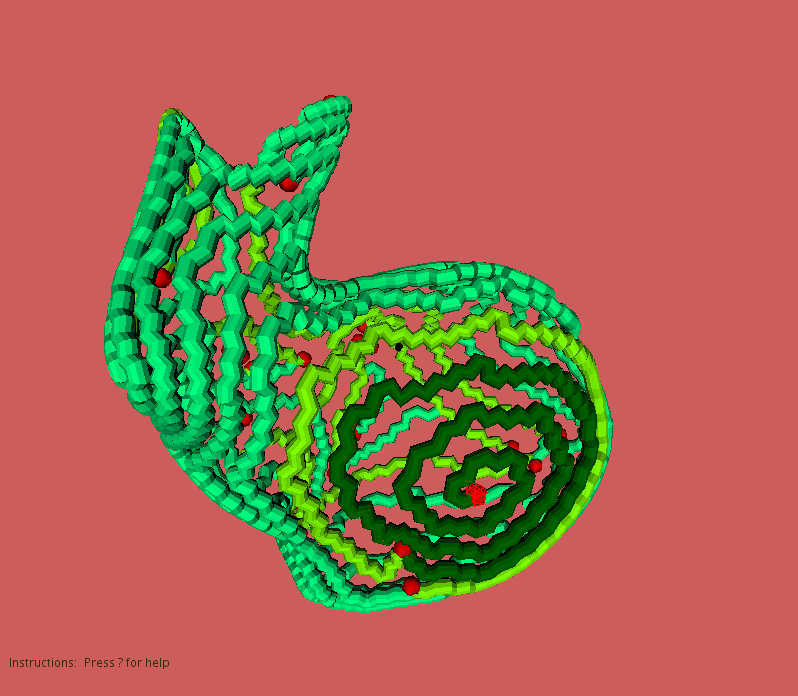
\includegraphics[height=80pt]{images/bunnyFront_pathAnimated.png} 
		   \label{fig:bunnyFrontPathAnimated}
          }
          \caption{Results with bunny.vts (front view)}
          \label{fig:bunnyFrontResult}
\end{figure}


% -------------------------------
% Bunny Back
\begin{figure}[h]
		\centering
		  \subfigure[Hamiltonian path (bunny back view)]{
		   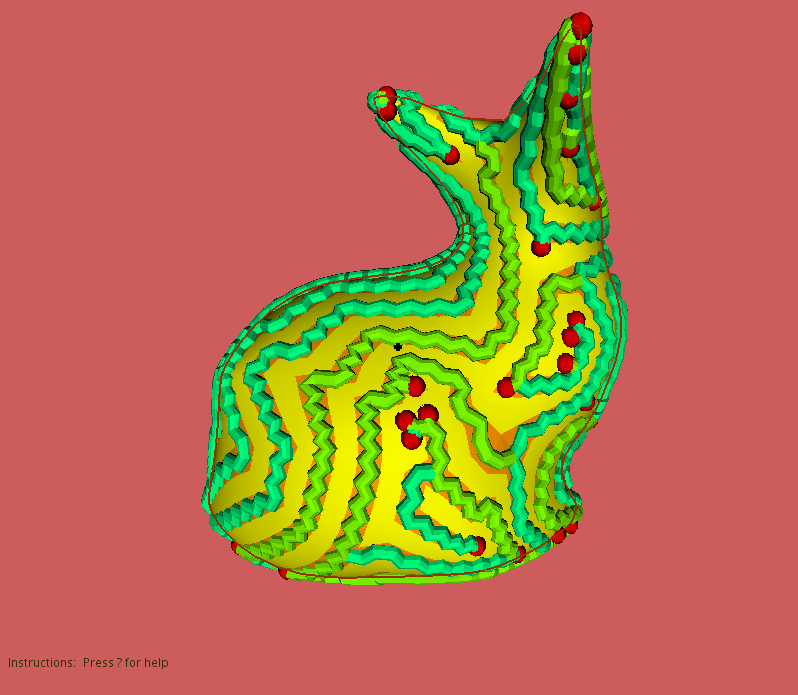
\includegraphics[height=80pt]{images/bunnyBack_path.png} 
		   \label{fig:bunnyBackPath}
          }		
		  \subfigure[Animation]{
		   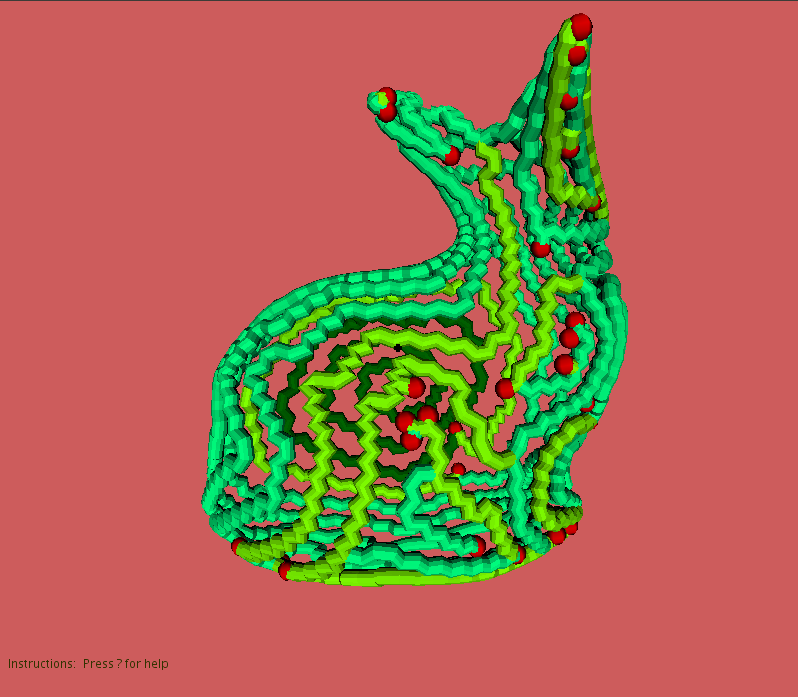
\includegraphics[height=80pt]{images/bunnyBack_pathAnimated.png} 
		   \label{fig:bunnyBackPathAnimated}
          }
          \caption{Results with bunny.vts (back view)}
          \label{fig:bunnyBackResult}
\end{figure}


%%%%%%%%%%%%%%%%%%%%%%%%%%%%%%%%%%%%%%%%%%%%%%%%%%%%%%%%%%%%%
% Bibliography
\bibliographystyle{IEEEtran}
\bibliography{references}

\end{document}
%%%%%%%%%%%%%%%%%%%%%%%%%%%%%%%%%%%%%%%%%%%%%%%%%%%%%%%%%%%%%